\subsubsection{Reduce}
\label{sssec:reduce}

\paragraph{Resumen} Esta función, al igual que los {\it mappers} se distribuye
automáticamente a través del sistema distribuido y trabaja sobre los archivos
intermedios que resultan de los mencionados {\it mappers}, los {\it workers}
que se encargan de realizar la etapa {reduce} leen estos archivos desde los
nodos de los {\it mappers} y se encargan de procesar los datos asociados a cada
clave-valor en orden.

Las etapas que son llevadas a cabo en la fase de {\it reduce}, se pueden ver en
la figura \ref{fig:mapreduce_reducer_phase}.


\begin{enumerate}
\setcounter{enumi}{1}
\item {\bf Asig. Reduce:} El {\it master} se encarga de distribuir la carga de
      reducer información correspondiente a la ubicación de los archivos 
      intermedios a los {\it workers} que trabajan como reducers.
\setcounter{enumi}{4}
\item {\bf Lectura Remota:} Al recibir la información del {\it master} acerca
      de la ubicación de los {\it archivos intermedios}, los {\it workers}
      proceden a la lectura de los mismos a través de RPC. El worker ahora
      procede a realizar las tareas de {\it reduce}.
\item {\bf Escritura:} Luego de haber procesado los datos de las claves que le
      fueron asignadas al {\it reducer}, este pasa a guardar los resultados a
      los archivos de salida {\it S1} y {\it S2}.
\end{enumerate}

\begin{figure}[h]
  \centering
  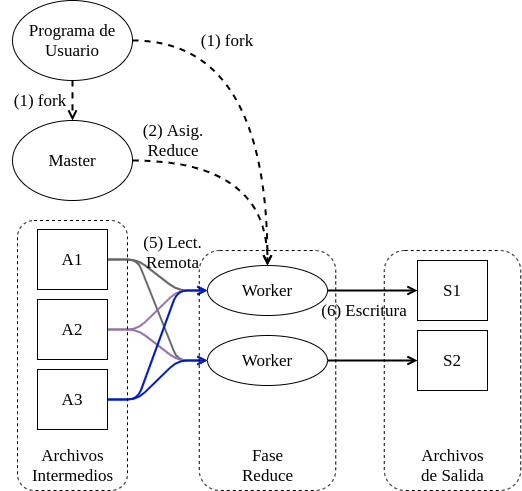
\includegraphics[width=0.75\linewidth]{figuras/MapReduce_reducer_phase.png}
  \caption{MapReduce: Fase {\tt reduce}}
  \label{fig:mapreduce_reducer_phase}
\end{figure}


